% Create pdf
% pdflatex --jobname=modules doc_tikz.tex

% Convert to png
% C:\Programme\gs\gs8.63\bin\gswin32.exe -dNOPAUSE -r400 -dEPSCrop -dGraphicsAlphaBits=4 -dTextAlphaBits=4 -sDEVICE=png16m  -sOutputFile=modules2.png -dBATCH modules.pdf

% C:\Programme\gs\gs8.63\bin\gswin32.exe -dNOPAUSE -r400 -g374x297 -dPDFFitPage -dEPSCrop -dGraphicsAlphaBits=4 -dTextAlphaBits=4  -sDEVICE=png16m -sOutputFile=modules3.png -dBATCH modules.pdf

% But in the end I used inkscape File/Export Bitmap and that was the best
% quality

\documentclass[10pt, a4paper]{article}

\usepackage[utf8]{inputenc}
\usepackage{pgf,tikz}
\pgfrealjobname{modules_int}

\usetikzlibrary{shapes.gates.logic.US,trees,positioning,arrows,petri}

%\parindent 0pt
%\parskip 1.5ex

\begin{document}

\beginpgfgraphicnamed{modules}
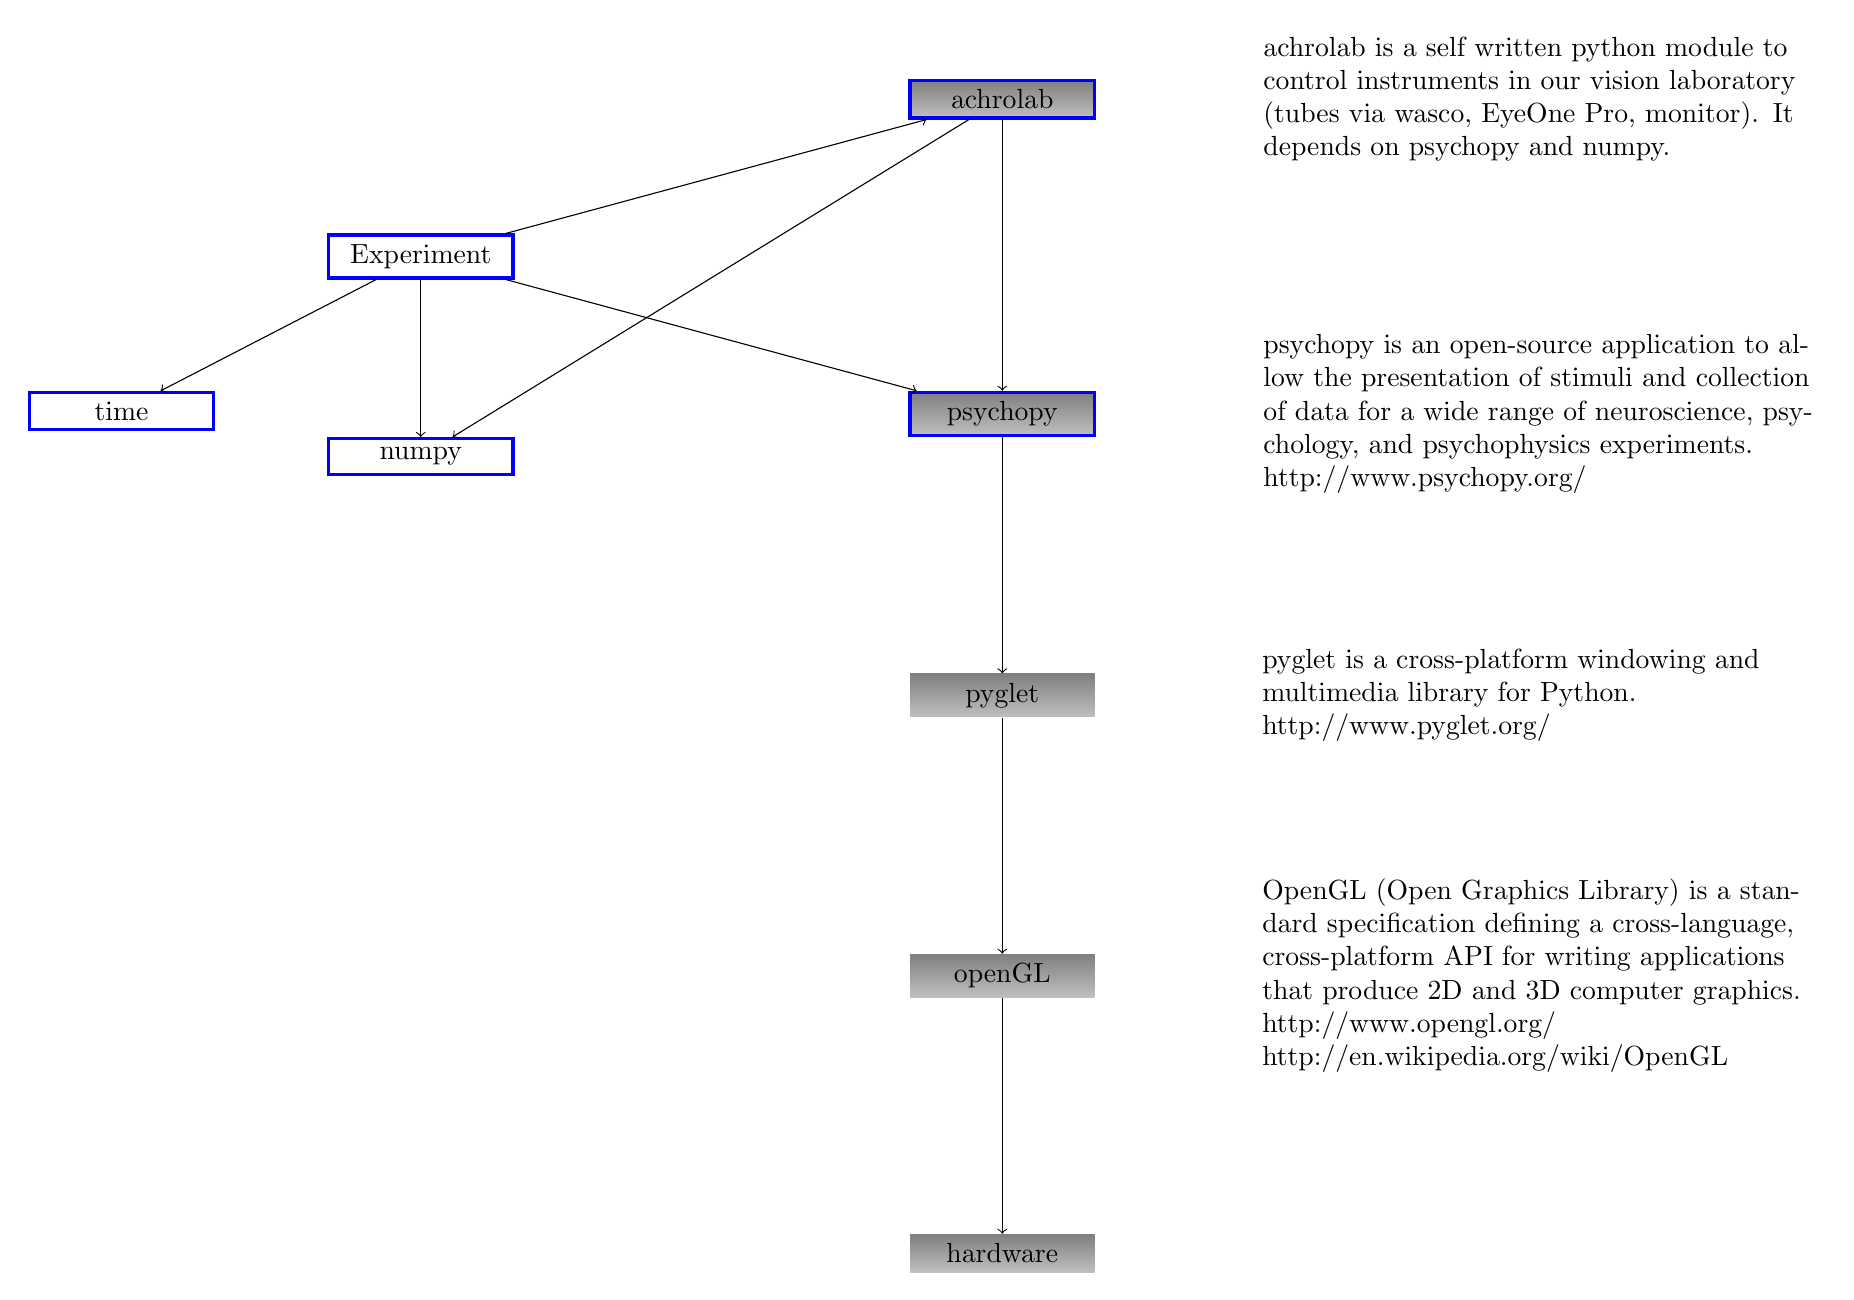
\begin{tikzpicture}
    \begin{scope}[node distance=2cm,
     	mynode/.style={rectangle, text width=6em, text centered, bottom color=lightgray},
     	mycol/.style={rectangle, draw=blue, text width=6em, text centered, very thick},
     	myboth/.style={rectangle, draw=blue, text width=6em, text centered, bottom color=lightgray, very thick},
        mylabel/.style={text width=20em}]
    \node [mycol] (exp)                              {Experiment};
    \node[mycol, below=of exp] (numpy) {numpy} edge [<-] (exp);
    % right branch
    \node [myboth] (vislab)[right=5cm of exp, yshift=2cm] {achrolab} edge [<-] (exp) edge [->] (numpy);
    \node [mylabel] (label1)[right=of vislab] {achrolab is a self written
    python module to control instruments in our vision laboratory (tubes via wasco, EyeOne Pro, monitor).
    It depends on psychopy and numpy.};
    \node [myboth] (psypy) [right=5cm of exp, yshift=-2cm]{psychopy} edge [<-] (exp) edge [<-] (vislab);
    \node [mylabel] (label2)[right=of psypy] {psychopy is an open-source application to allow the presentation
    of stimuli and collection of data for a wide range of neuroscience, psychology, and psychophysics experiments.\\http://www.psychopy.org/};
    \node [mynode] (pyglet)[below=3cm of psypy]           {pyglet} edge [<-] (psypy);
    \node [mylabel](label3)[right=of pyglet] {pyglet is a cross-platform windowing and multimedia library for Python.\\http://www.pyglet.org/};
    \node [mynode] (opengl)[below=3cm of pyglet]          {openGL} edge [<-] (pyglet);
    \node [mylabel](label4)[right=of opengl] {OpenGL (Open Graphics Library) is a standard specification defining a cross-language,
    cross-platform API for writing applications that produce 2D and 3D computer graphics.\\http://www.opengl.org/\\http://en.wikipedia.org/wiki/OpenGL};
    \node [mynode] (hard)[below=3cm of opengl]            {hardware} edge [<-] (opengl);
    % left branch
    \node[mycol, below left=of exp] (time) {time} edge [<-] (exp);
    %\node[myboth, above=of exp] (rpy2) {rpy2} edge [<-] (exp) edge [<-] (vislab);
    \end{scope}
\end{tikzpicture}
\endpgfgraphicnamed

\end{document}

